\documentclass[]{witrman}

\usepackage{xfrac}  % for 1/2 turn later in the document

\setsecnumdepth{none}
\title{DJ TRAINER GUIDE}
\date{FALL 2018}
\renewcommand{\TitlepageGraphic}{images/titlepage}

\newcommand{\makehomework}[1]{%
\vspace{1mm}
\rule{\textwidth}{1pt}
\textbf{Homework}:\\
#1\\
\rule[2mm]{\textwidth}{1pt}
}

\begin{document}

\maketitle

\maketoc{}

\setpagebg{}

\chapter{Shadowing}

Welcome your trainee to the wonderful world of DJing at WITR\@. Talk about their
music passions and show off the mixing board.

\makehomework{Study the All Member Manual.  (Send your trainee
\href{https://github.com/WITR-Radio/manuals/releases}{a copy of the
manual} if they don't already have it.)}


\chapter{Session 1}

Say hello to your new trainee, introduce yourself, tell them a bit about your
time at the station, and ask about your trainee's music tastes.

\subsection{Music}

Show your trainee the library and have them pick out their own set of 3 tracks.
Play the trainee's tracks while walking them through the basics of what you're
doing.

\subsection{Equipment}

Set up your next set through Rivendell and show the trainee how to preview
songs.  Explain how the online song logger works, how to manually edit logger
entries, and how the downstairs paper logs should be filled out.

\subsection{On-Air}

Offer for your trainee to join you on the next mic break.  They may need
encouragement to get on the mic, but don't press them too much if they're not
comfortable with the idea of talking on-air yet.

\makehomework{Review a full-length album.  Bring it to your next session.}


\chapter{Session 2}

Give your trainee a complete rundown of the mixing board, and tell them about
various DJ styles and personality types.

\subsection{Music}

Ask your trainee to pick out two full sets, have them play their own tracks, and
explain how to maintain a flow between different sets.  Show them the different
imaging options and how we can use imaging to transition between different music
styles.

\subsection{Equipment}

Explain what each of the channels on the board does and how to keep your eye on
the levels.  Don't forget to mention to your trainee that turning on a CD or
vinyl input will start track.  Also explain how to preview tracks through the
headphones or monitors.  Teach them how to crossfade between two songs.

\subsection{On-Air}

Explain the different elements of a mic break: elements that \textbf{must} be
covered, elements that are up to the DJ's discretion, and the list of things
that can \textbf{never} be said on-air.  Show your trainee how to physically do
a mic break (both the tech and how to speak into a mic).  Have them do a mic
break in between their sets.

\makehomework{Listen to a full, 2-hour Pulse of Music show and write down a few
comments on the music played and the DJ's mic breaks.}


\chapter{Session 3}

Explain each function of RDLibrary and RDAirPlay to your trainee.  Encourage
them to check out (and review) new music.  Tell them the structure that a Pulse
of Music show must follow and talk to them about the comments they wrote on the
show they listened to last week.

The Pulse of Music format: 1 recurrent, 2 features, and 1 double shot per hour;
50\% new bin balance during the 2 hour show; and Pulse of Music imaging
throughout.

\subsection{Music}

Have your trainee create a set on RDAirPlay with a track from each of the
following bins: Library, New Bin, Feature, and Recurrent.  Have them play 3 more
sets all on CDs.

Show them where in the office to find new CDs, how to check them out, and
explain to them the general review format that we follow (below).  Show them an
example of a good and a bad review.  Tell your trainee about a band you like
that you first discovered while reviewing one of their CDs.

\subsection{Equipment}

RDLibrary:
\begin{tightitemize}
    \item The Bins
    \item Searching the library
    \item Using the `only show first 100' checkbox
\end{tightitemize}

RDAirPlay:
\begin{tightitemize}
    \item Delete or move a track
    \item Track talk-markers
    \item Loading the logs (this is \textbf{crucial}, especially the distinction
        between FM and Underground logs)
    \item Auto/Manual modes
    \item How to recover from an RDAirPlay crash
\end{tightitemize}

\subsection{On-Air}

Ask your trainee if they've thought about what style they want to have as a DJ
and brainstorm some DJ names.

\makehomework{Review a full-length album.  Bring to the next session.}


\chapter{Session 4}

Get your trainee comfortable with mic breaks.  Look over the CD review they
wrote and give critiques.

\subsection{Music}

Pick out a couple of sets of your own and show your trainee how to research
background information to include in a mic break.

\subsection{Equipment}

Show your trainee how to fill out support tickets and go over what situations
constitute an emergency.

\subsection{On-Air}

Coach your trainee on how to convey their personality while on mic (smiling
while talking, pretending they're talking to a friend, throwing in some humor,
etc.).

\makehomework{Study the DJ Training Manual.}


\chapter{Session 5}

Teach your trainee how to use the turntables.  Time to let them spread their
wings and fly!

If your trainee isn't already a member of the family, try to get them involved
in the station's social circle.

\subsection{Music}

Ask your trainee to pick out a vinyl album or two from the library to play.

\subsection{Equipment}

Teach your trainee how to find and play vinyls:
\begin{tightitemize}
    \item Using the Vinyl Bible on the DJ portal
    \item Cleaning and maintenance of the turntable
    \item Board operation for turntable channel
    \item Previewing a track
    \item Cuing up a track ($\sfrac{1}{2}$ turn)
\end{tightitemize}

\subsection{On-Air}

Have your trainee DJ for the whole hour.  Supervise them and provide guidance if
they need it.  Write down your notes to go over with them later and let them
know what habits would hurt their demo score.

\begin{center}
    %\caption{Your trainee is growing up fast!}
    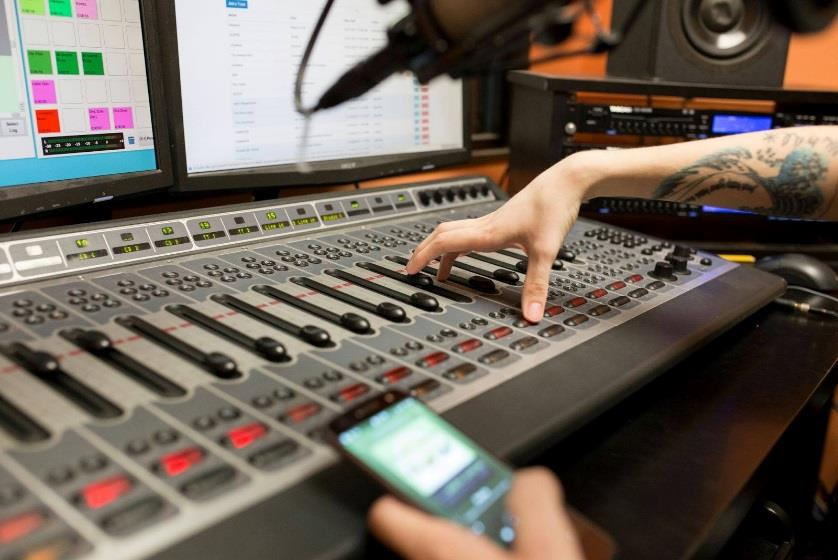
\includegraphics[width=8cm]{images/console}
\end{center}

\makehomework{Pass the DJ Test.}


\chapter{Session 6}

What do we do when s--- hits the fan?

If your trainee did not pass their DJ test, ask the Programming Director to see
your trainee's test and review their mistakes with them.

\subsection{Music}

If a track says an FCC-violating lyric:
\begin{tightenumerate}
    \item Hit the dump button
    \item If you have time, look up the full lyrics to determine if there are
        any more swears in the song
    \item If there's no time, or if the song has more profanity, fade the song
        out into imaging and cue a new song
    \item Mark the track as an FCC violation on the label
    \item Email the Music Director and Programming Director and describe the
        violation
\end{tightenumerate}

\subsection{Equipment}

If RDAirPlay or RDLibrary crash:
\begin{enumerate}
    \item Have at least 1 CD cued up in the CD player for exactly this situation
    \item Play the Emergency Music
    \item Force close RDAirPlay
    \item Start RDAirPlay and RDSecondPanel back up
    \item Load the log and resume playing tracks as usual
\end{enumerate}

\subsection{On-Air}

Have your trainee DJ for the whole hour.  Supervise, but try not to give them
advice if they get flustered.  Emphasize the need for them to keep calm and
level-headed in these situations.  Make notes on the show and review with them
afterward.

\makehomework{Listen to the playback from another trainee's show.  Make notes on
what they did well or did poorly.  Write down any Pulse of Music structure
violations you notice.}


\chapter{Session 7}

Get your trainee in the groove of a regular show.

\subsection{On-Air}

Have your trainee DJ for the whole hour.  Supervise them and provide guidance if
they need it.  Write down your notes to go over with them later and let them
know what habits would hurt their demo score.

\makehomework{Review 2 full-length albums.}


\chapter{Session 8}

Time to see if your trainee will sink or swim.

\subsection{On-Air}

Have your trainee DJ for the whole hour.  Sit in another room and monitor the
Studio A underground feed.  This is essentially a test run for your trainee's
demo.  If you are not completely confident in their ability to pass the demo,
let your trainee do a typical supervised show the upcoming week, then have them
try a solo show again the following week.  Write down your notes to go over with
them later.

\makehomework{Record your DJ demo.}


\chapter{Finish Line}

Your trainee is now all grown up and ready to leave the nest!  Make sure to
congratulate them on their demo.

\makefooter{}

\end{document}
